%!TEX root = ../thesis.tex

\section{ロボットアームの構造設計}
要求仕様に基づき,6軸のロボットアームを設計した(図\ref{fig:arm_design}参照).設計にはAutodesk社のInventor 2023\cite{inventor:online}を使用した.リンク部には,板金部品とアルミフレームを採用し,シリアルリンク機構を構成している.また,専門的な技術を必要とせず,ネジ締結のみで組立が可能な設計を採用した.
設計したロボットアームのデータはGitHub上で公開しており,自由に閲覧・利用が可能である(https://github.com/open-rdc/OfficeRobot).

本節では,ロボットアームの構造設計について述べる.なお,本設計は次節で実施する強度確認を踏まえた最適化が前提であり,現時点で示す内容は仮のものである.設計した板金部品についても,構造解析結果に基づいて形状変更が行われる予定である.

\begin{figure}
  \centering
  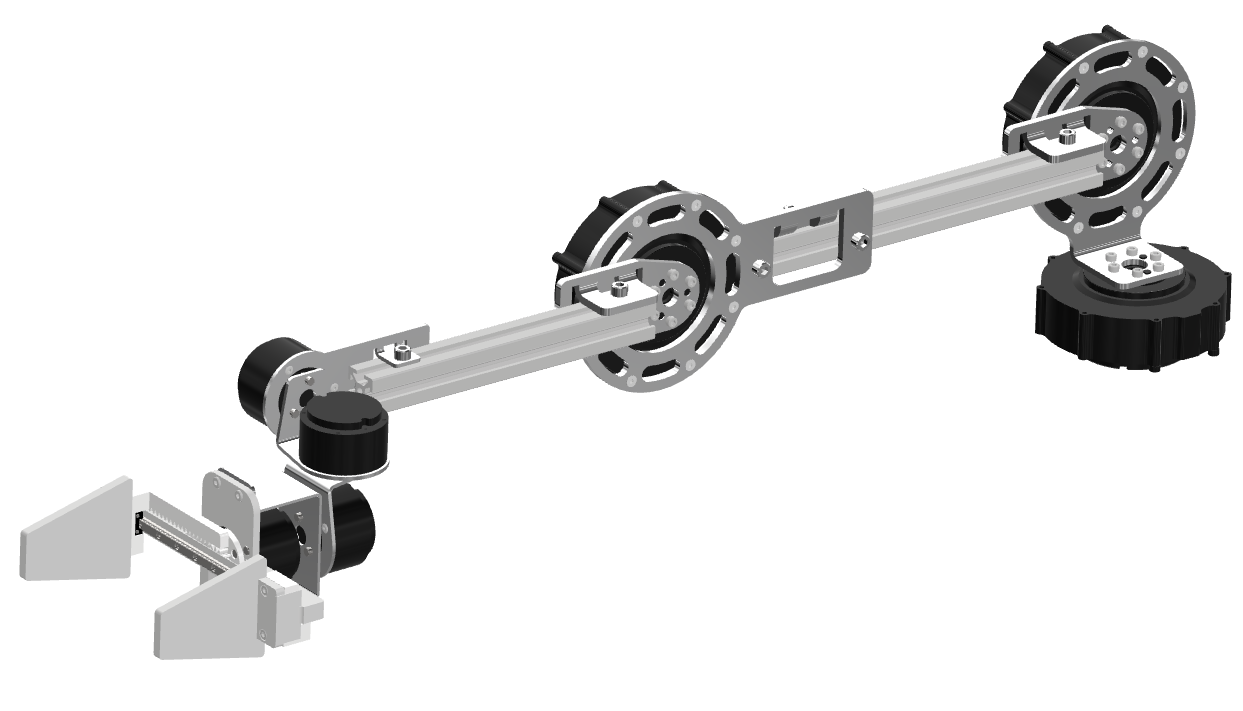
\includegraphics[width=10cm]{images/design/arm_design.png}
  \caption{The mechanical design of the robot arm}
  \label{fig:arm_design}
\end{figure}
\clearpage

\subsection{軸配置}
図\ref{fig:zikuhai}にロボットアームの軸配置を示す.要求仕様に基づき,肩に2軸,肘に1軸,手首3軸を配置している.また,エンドエフェクタの開閉には1軸を用いている.
\begin{figure}
  \centering
  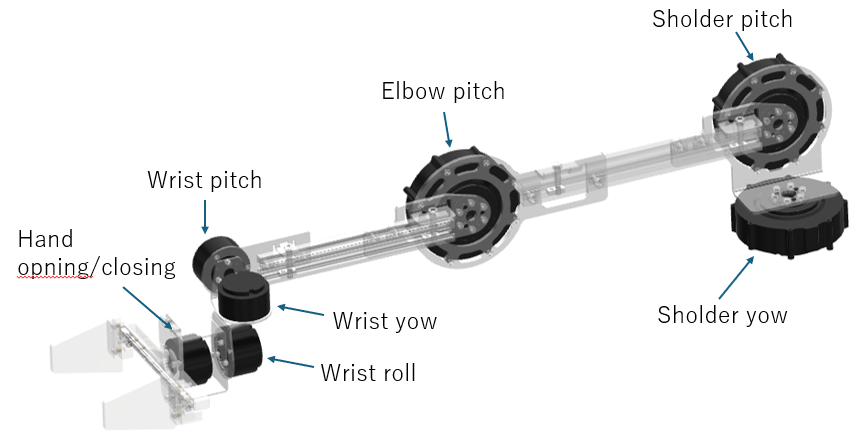
\includegraphics[width=10cm]{images/design/skelton.png}
  \caption{Axis configuration of the robot arm.}
  \label{fig:zikuhai}
\end{figure}

\subsection{軸間距離}
図\ref{fig:link_length}にロボットアームのアームリーチとリンク長を示す.アームリーチの仕様は510㎜から750mmであり,本ロボットアームでは仕様範囲内の660㎜を採用した.肩から肘,肘から手首のリンク長の比率については,人間の腕を比率を参考に設定した\cite{humanarm:online}.
\begin{figure}
  \centering
  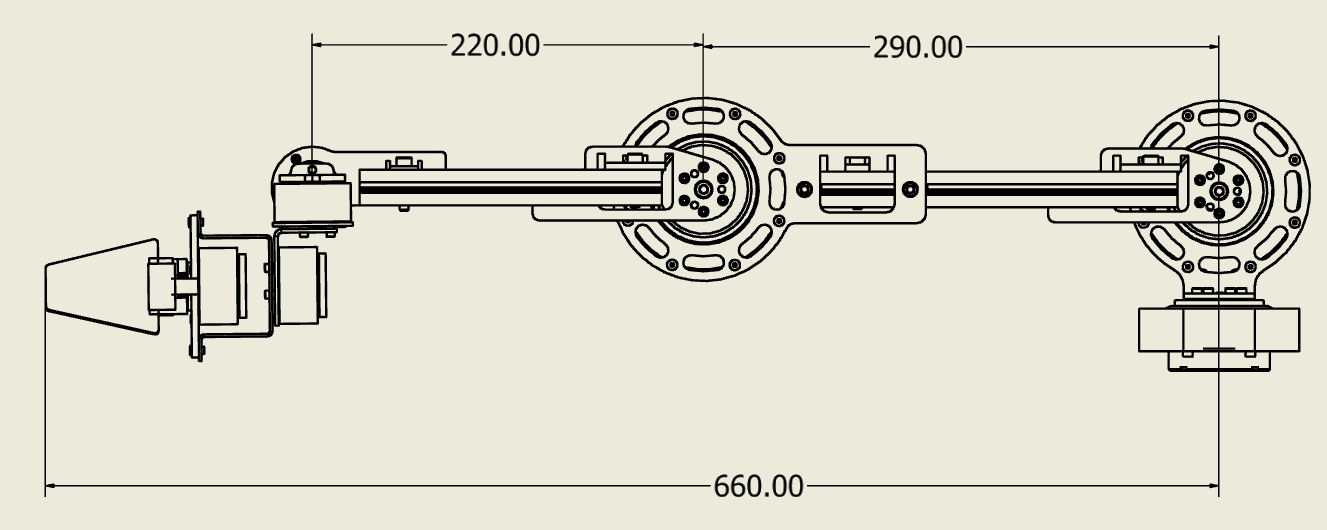
\includegraphics[width=10cm]{images/design/link_length.png}
  \caption{Arm reach and link length}
  \label{fig:link_length}
\end{figure}
\clearpage

\subsection{可搬重量}
設定したアームリーチで,仕様である500gの可搬重量を定格トルクで確保できるかを確認する.また,最大トルク時の可搬重量についても計算を行う.
肩ピッチ軸のQDDモータ(SteadyWin GIM8108-8)の定格トルクは7.5Nm,最大トルクは22Nmである.アームを伸ばした際に,自重を支えるために必要なトルクを算出し,常時把持することのできる物体の重量と,瞬間的に把持することのできる物体の重量を求める.
\subsubsection{自重を支える為に必要なトルク}
図\ref{fig:CoG}にアームの重心を示す.アームの重心は肩ピッチ軸から0.334mの位置にあり,アームの重さは1.31kgである.重力加速度を9.8m/s$^2$とすると,肩ピッチ軸にかかるトルク$T$は次のように求められる.
\begin{equation}
  T = 1.31 \times 9.8 \times 0.334 = 4.2 Nm
\end{equation}
\begin{figure}[h]
  \centering
  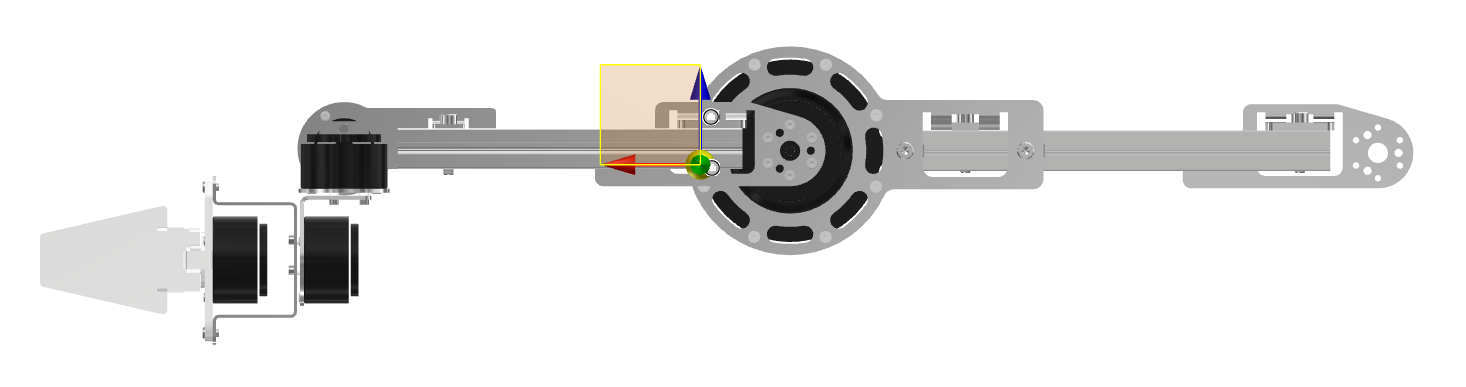
\includegraphics[width=10cm]{images/design/CoG.png}
  \caption{Center of gravity}
  \label{fig:CoG}
\end{figure}

\subsubsection{常時把持することのできる物体の重量}
アームの定格トルクから,自重を支える為に必要なトルクを引くと3.3Nmであり,肩ピッチ軸から手先までの距離は0.66mである.したがって,常時把持することのできる物体の重量$m$は次のように求められ,仕様の500g以上の可搬重量を満たしていることが確認できる.
\begin{equation}
  m = 3.3 / (9.8 \times 0.66) = 0.51kg
\end{equation}

\subsubsection{瞬間的に把持することのできる物体の重量}
同様に,最大トルクから自重を支える為に必要なトルクを引くと17.8Nmである.したがって,瞬間的に把持することのできる物体の重量$M$は次のように求められる.
\begin{equation}
  m = 17.8 / (9.8 \times 0.66) = 2.75kg
\end{equation}

\subsection{可動範囲}
図\ref{fig:arm_short}および図\ref{fig:arm_long}に,エンドエフェクタを水平に保った際のロボットアームの最小可動範囲と最大可動範囲を示す.最小可動範囲は,部品同士が干渉せずに動作可能な最小の範囲を指し,最大可動範囲はアームを最大まで伸ばした際の動作可能範囲を示している.

現行の最小可動範囲では,狭小エリアなど台車の移動に制限が生じる状況への対応が難しいと予想される.そこで,机の片付け作業を想定し,机と缶を模したCADモデルを使用して作業領域の確認を行った.
\begin{figure}[h]
  \centering
  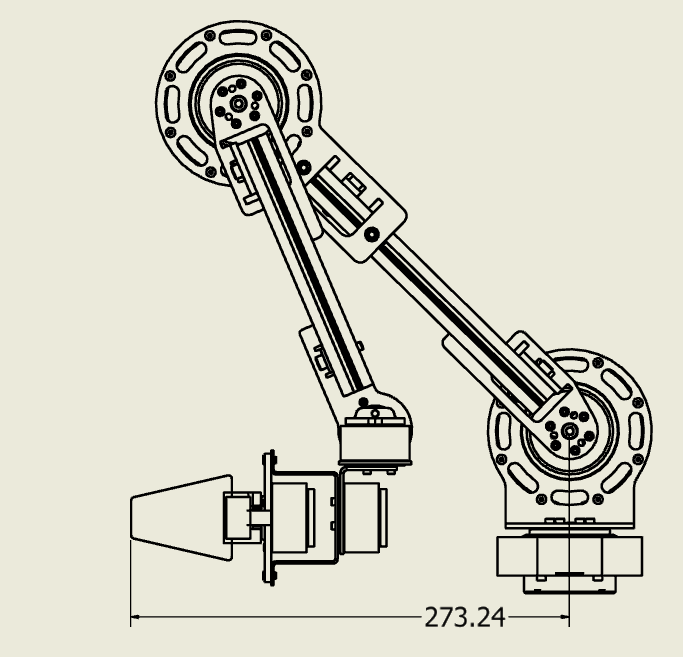
\includegraphics[width=10cm]{images/design/arm_short.png}
  \caption{Minimum range of motion}
  \label{fig:arm_short}
\end{figure}

\begin{figure}[t]
  \centering
  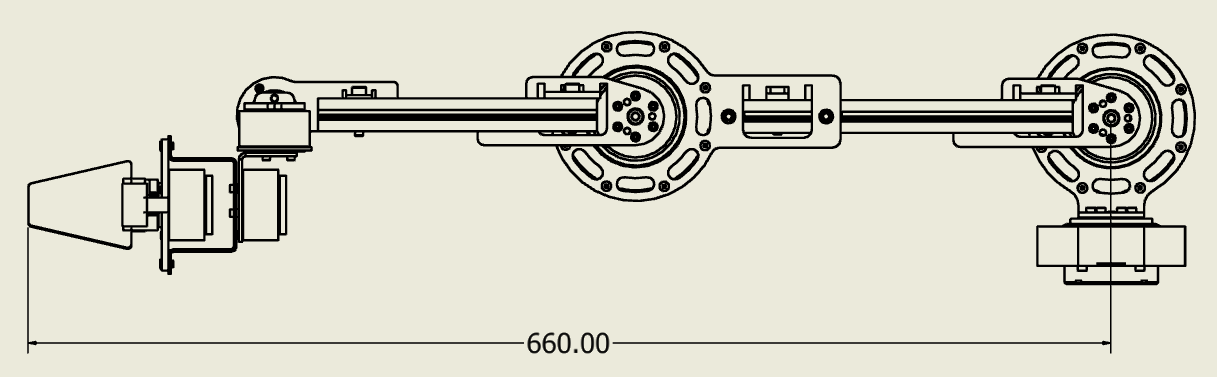
\includegraphics[width=10cm]{images/design/arm_long.png}
  \caption{Maximum range of motion}
  \label{fig:arm_long}
\end{figure}
\clearpage

図\ref{fig:arm_size}にロボットアーム,机,缶,の位置関係を示し,
図\ref{fig:syokisisei}にロボットの初期姿勢を示す.図\ref{fig:syokisisei}における黄色の点を原点(x, y)=(0, 0)とし,図\ref{fig:arm_move}の(a)から(h)の順にアームを動かして手先位置を計測した.なお,エンドエフェクタの角度は図\ref{fig:syokisisei}状態から変更せず,缶を正面から把持することを想定した.缶の設置位置を,机の縁から500㎜以内と仮定し,図\ref{fig:arm_move}の(d)は,x = -500,(f)は,x = 500 のときの最大可動範囲を示している.

計測したアームの手先位置を図\ref{fig:prot}に示す.
図\ref{fig:prot}の(b)は,図\ref{fig:prot}の(a)の視点から観測した手先位置(星印)をプロットしたものであり,おおよその作業領域を表している.図\ref{fig:prot}の(b)より,ロボットアームに近い位置でアクセスできない領域が存在することが確認された.

会議室など,オフィスロボットが十分なスペースを確保できる環境では,現在のロボットアームでも対応可能である.しかし,移動が制限される狭小エリアでは作業が困難になる可能性がある.したがって,今後の課題として,作業領域の拡大が必要である.

\begin{figure}[h]
  \centering
  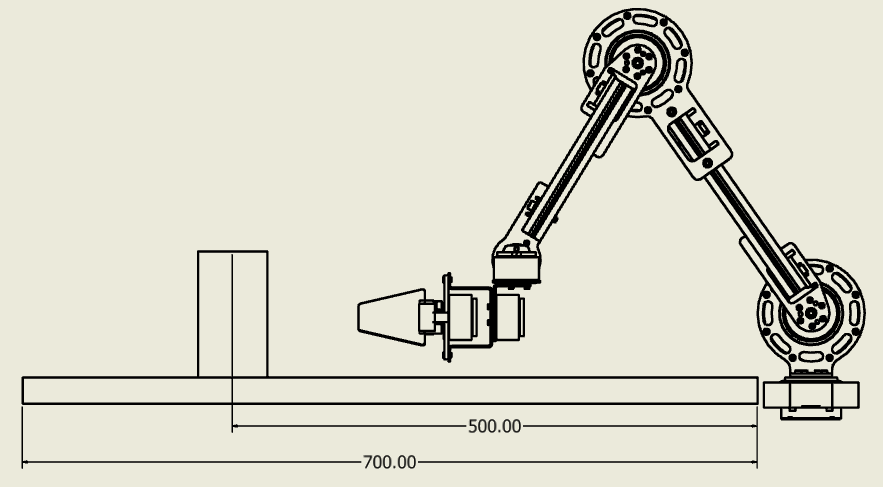
\includegraphics[width=10cm]{images/design/hikaku.png}
  \caption{Positional relationship between desk, can and robot arm.}
  \label{fig:arm_size}
\end{figure}

\begin{figure}
  \centering
  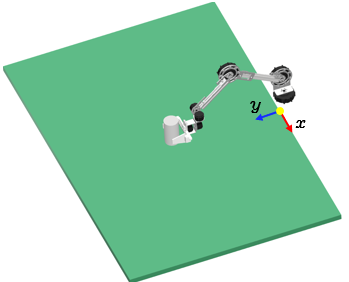
\includegraphics[width=10cm]{images/design/syoki.png}
  \caption{Initioal position of robot arm}
  \label{fig:syokisisei}
\end{figure}
\begin{figure}
  \centering
  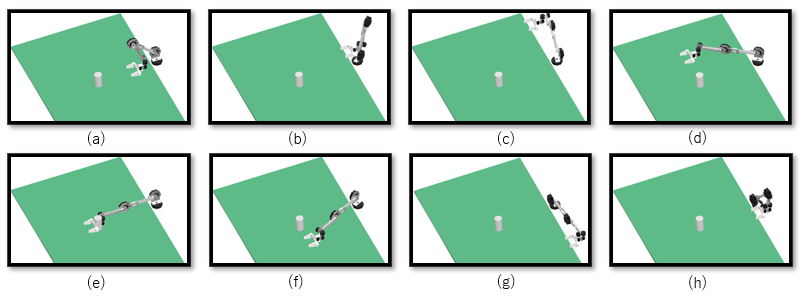
\includegraphics[width=13cm]{images/design/arm_move.png}
  \caption{Checking the working area of the robot arm}
  \label{fig:arm_move}
\end{figure}
\begin{figure}
  \centering
  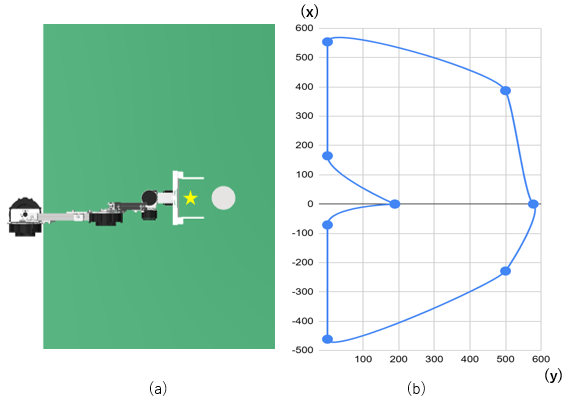
\includegraphics[width=10cm]{images/design/prot.png}
  \caption{Results of measuring the hand position of the robot arm shown in the figure\ref{fig:arm_move}.}
  \label{fig:prot}
\end{figure}
\clearpage
